\section{Two-Moment Model}\label{se:Two-MomentModel}

\subsection{Transport Equations}
We consider neutrino transport through a static background, and include neutrino-matter interactions due to emission, absorption, and isoenergetic scattering.
After scaling to dimensionless units, the Boltzmann equation can be written as
\begin{equation}
  \pd{f}{t}+\vect{\ell}\cdot\nabla f
  =\f{1}{\tau}\,\cC(f),
  \label{eq:boltzmann}
\end{equation}
where the distribution function $f = f(\omega,\varepsilon,\vect{x},t)$ gives the number of neutrinos propagating in the direction $\omega\in\bbS^{2}$, with energy $\varepsilon\in\bbR^{+}$, at position $\vect{x}\in\bbR^{3}$ and time $t\in\bbR^{+}$.  
$\vect{\ell}(\omega)\in\bbR^{3}$ is the unit vector parallel to the neutrino three-momentum: $\vect{p}=\varepsilon\,\vect{\ell}$.
On the right-hand side, $\tau$ is a collision time scale.  
In opaque regions, where neutrinos have frequent interactions with the background, $\tau\ll1$.  
In transparent regions, where neutrinos rarely interact and stream freely, $\tau\gg1$.
The collision term, $\cC(f)$, which models emission, absorption, and isoenergetic scattering is given by
\begin{equation}
  \cC(f)=\xi\,\big(\,f_{0}-f\,\big)
  +(1-\xi)\,\big(\,\f{1}{4\pi}\int_{\bbS^{2}}f\,d\omega-f\,\big),
  \label{eq:collisionTerm}
\end{equation}
where $\xi = \sigma_{\Ab} / (\sigma_{\Ab}  + \sigma_{\Scatt} )$ is the ratio of the absorption opacity $\sigma_{\Ab}$ to the total opacity.  
The scattering opacity is $\sigma_{\Scatt}$.  
The limit $\xi = 1$, when $\sigma_{\Scatt} = 0$, corresponds to pure absorption, while $\xi = 0$, when $\sigma_{\Ab} = 0$, corresponds to pure scattering.  
The equilibrium distribution function for neutrinos is given by the Fermi-Dirac distribution:
\begin{equation}
  f_{0}(\vect{z})=\f{1}{e^{(\varepsilon-\mu(\vect{x}))/T(\vect{x})}+1}, 
  \label{eq:fermiDirac}
\end{equation}
where $\vect{z}:=\{\varepsilon,\vect{x}\}$, $T$ is the material temperature in energy units and $\mu$ is the neutrino chemical potential.
Both $T$ and $\mu$ depend on the spatial position $\vect{x}$.

\subsection{Two-Moment Model}

Approximate solutions to the Boltzmann equation, Eq.~\eqref{eq:boltzmann}, can be found by solving the two-moment model.
To this end, define the angular moments of the distribution function as follows:
\begin{equation}
  \big\{\,\cJ,\vect{\cH},\vect{\cK}\,\big\}(\vect{z},t)
  =\f{1}{4\pi}\int_{\bbS^{2}}f(\omega,\vect{z},t)\,\{\,1,\vect{\ell},\vect{\ell}\otimes\vect{\ell}\,\}\,d\omega.
  \label{eq:angularMoments}
\end{equation}  
The zeroth moment, $\cJ$, is referred to as the particle density.  
The first moment, $\bcH$, is the particle flux, and the second moment, $\bcK$, is proportional to the stress tensor.  
By integrating Eq.~\eqref{eq:boltzmann} over the momentum-space angular dimension we obtain equations for the zeroth and the first moments:
\begin{equation}
  \pd{\vect{\cM}}{t}+\nabla\cdot\vect{\cF}=\f{1}{\tau}\,\vect{\cC}(\vect{\cM}),
  \label{eq:momentEquations}
\end{equation}
with $\vect{\cM}=(\cJ,\vect{\cH})^{T}$, $\vect{\cF}=(\vect{\cH},\vect{\cK})^{T}$, and
\begin{equation}
  \vect{\cC}(\vect{\cM})=\vect{\eta}-\vect{\cD}\,\vect{\cM},
  \label{eq:collisionTermMoments}
\end{equation}
where $\vect{\eta}=(\xi\,f_{0},\vect{0})^{T}$, $\vect{\cD}=\mbox{diag}(\xi,\vect{I})$, and
$\vect{I}$ is the identity matrix.
Hence, the process of solving the Boltzmann equation, Eq.~\eqref{eq:boltzmann}, for the neutrino distribution function $f(\omega,\vect{z},t)$, is replaced by solving the two-moment equations for the neutrino number density, $\cJ(\vect{z},t)$, and flux, $\bcH(\vect{z},t)$.  

\subsection{Algebraic Closures}

The moment equation for $\bcH$ involves the higher moment $\bcK$ and the two-moment model is open.  
To close the two-moment model, we consider algebraic closures.  
For the two-moment model, algebraic closures give an approximation to $\bcK$ using the lower moments:
\begin{equation}
  \bcK = \vect{k} \cJ,
\end{equation}
where $\vect{k}$ is the Eddington tensor.  
By assuming that the distribution function is symmetric about a preferred direction $\widehat{\vect{h}}=\vect{\cH}/|\vect{\cH}|$, Levermore~\cite{levermore_1984} proposed a simple form for the Eddington tensor:
\begin{equation}
  \vect{k}=\f{1}{2}\big[\,\big(1-\chi\big)\,\vect{I}+\big(3\,\chi-1\big)\,\widehat{\vect{h}}\otimes\widehat{\vect{h}}\,\big],
  \label{eq:eddingtonTensor}
\end{equation}
where $\chi=\chi(\cJ,|\vect{\cH}|)$ is the Eddington factor.  
Thus, the two-moment model is closed by specifying the scalar $\chi$ in terms of $\cJ$ and $|\vect{\cH}|$.  

\subsection{Constraints on the Moments}

Neutrinos are fermions and obey the Pauli exclusion principle.  
Because of this, the neutrino distribution function is bounded; i.e.~$f \in [0,1]$.
As a result, the angular moments $\cJ$ and $\vect{\cH}$ and the Eddington factor $\chi$ satisfy the following bounds~\cite{levermore_1984,lareckiBanach_2011,kershaw_1976,shohatTamarkin_1943}: 
\begin{align}
\cJ \in[0,1], \quad &(1-\cJ)\cJ-|\vect{\cH}| \geq 0, \label{eq:MomentsBounds} \\
  \chi_{\mbox{\tiny min}}
  =\max\big(1-\f{2}{3\cJ},h^{2}\big)
  \leq & \chi \leq \min\big(1,\f{1}{3\cJ}-\f{\cJ}{1-\cJ}h^{2}\big)=\chi_{\mbox{\tiny max}},
  \label{eq:eddingtonFactorBounds}
\end{align}
where $h = |\bcH|/\cJ$ is the flux factor.  

The constraints in Eq.~\eqref{eq:MomentsBounds} define realizable moments $\bcM$.  
For fermions, realizable moments can only be constructed from a distribution satisfying the bounds $f \in [0,1]$.  
Moreover, the set of realizable moments is convex: let $\cR$ be the realizability set and $\bcM_{1}, \bcM_{2} \in \cR$, then $\lambda \bcM_{1} + (1-\lambda)\bcM_{2} \in \cR$ for any $\lambda \in [0,1]$~\cite{chu_etal_2018}.
As we will see later in Section~\ref{se:SpatialDiscretization}, this convexity makes it possible to design a realizability-preserving discretization for solving the two-moment model numerically.

The inequalities in Eq.~\eqref{eq:eddingtonFactorBounds} deserve further attention.  
They are as important as those in Eq.~\eqref{eq:MomentsBounds}, in maintaining consistency of the two-moment model with respect to Fermi-Dirac statistics.  
When designing a numerical scheme for the two-moment model that maintains realizable $\bcM$, it is also necessary for the Eddington factor to satisfy the bounds in Eq.~\eqref{eq:eddingtonFactorBounds}.  

However, recently reported CCSN simulations using two-moment neutrino transport with algebraic closures have employed Eddington factors that can violate the bounds in Eq.~\eqref{eq:eddingtonFactorBounds}.  
As examples, we consider the Eddington factors discussed in~\cite{murchikova_etal_2017}, where the suitability of several algebraic closures for two-moment neutrino transport was evaluated.  
In Fig.~\ref{fig:EddingtonFactorsWithDifferentClosure}, we plot the Eddington factor versus the flux factor for two occupancies: $\cJ = 0.1$ (low occupancy) and $\cJ = 0.9$ (high occupancy).  
Of the algebraic closures plotted, few satisfy the bounds on the Eddington factor in Eq.~\eqref{eq:eddingtonFactorBounds}.  
Kershaw~\cite{kershaw_1976}, Wilson~\cite{wilson_1975,leblancWilson_1970}, Levermore~\cite{levermore_1984}, Minerbo~\cite{minerbo_1978}, and Janka~2~\cite{janka_1992} closures may work fine when the occupancy is low.  
When the occupancy is high, the Eddington factor due to these closures exceeds the upper bound for Fermi-Dirac statistics.  
The Eddington factor of Janka~1~\cite{janka_1991} may violate both the upper and lower bound on the Eddington factor.  
Only the closure due to Cernohorsky~\&~Bludman~\cite{cernohorskyBludman_1994} satisfies both the upper and lower bounds.  
This is not surprising as this is the only closure based on Fermi-Dirac statistics.  
Although the Levermore and Minerbo closures do not satisfy the bounds in Eq.~\eqref{eq:eddingtonFactorBounds}, they are widely used in simulations of neutrino transport in CCSNe and compact binary mergers; e.g., O'Connor \& Couch~\cite{oConnorCouch_2018}, Pan et al.~\cite{pan_etal_2018}, Glas et al.~\cite{glas_etal_2018}, Just et al.~\cite{just_etal_2018}, and Foucart et al.~\cite{foucart_etal_2015} use the Minerbo closure, while Vartanyan et al.~\cite{vartanyan_etal_2018}, Cabezon et al.~\cite{cabezon_etal_2018}, Kuroda et al.~\cite{kuroda_etal_2016}, and Fujibayashi et al.~\cite{fujibayashi_etal_2017} use the Levermore closure.  
When employing these closures in conditions of high occupancy, a numerical scheme may evolve the moments outside the realizable domain of Fermi-Dirac statistics given in Eq.~\eqref{eq:MomentsBounds}.
If this were to happen, the update step may give $\cJ>1$.
Considering the fact that the collision term contains blocking factors --- i.e.~$(1-\cJ)\times$ something positive --- $\cJ > 1$ would change the blocking factors' sign, and it would be difficult to predict the impact of the subsequent induced errors on the simulation outcome.
Besides, even with the simplified collision term Eq~\ref{eq:collisionTermMoments}, $\cJ>1$ could result in information loss (such as loss to the neutrino distribution for the groups that exceed the bounds), closure failure, and other unpredictable consequences.
If treatments are developed to map the unrealizable moments into the realizable domain, they should be developed to conserve lepton number, energy, and momentum.

\begin{figure}[h]
  \centering
  \begin{tabular}{cc}
    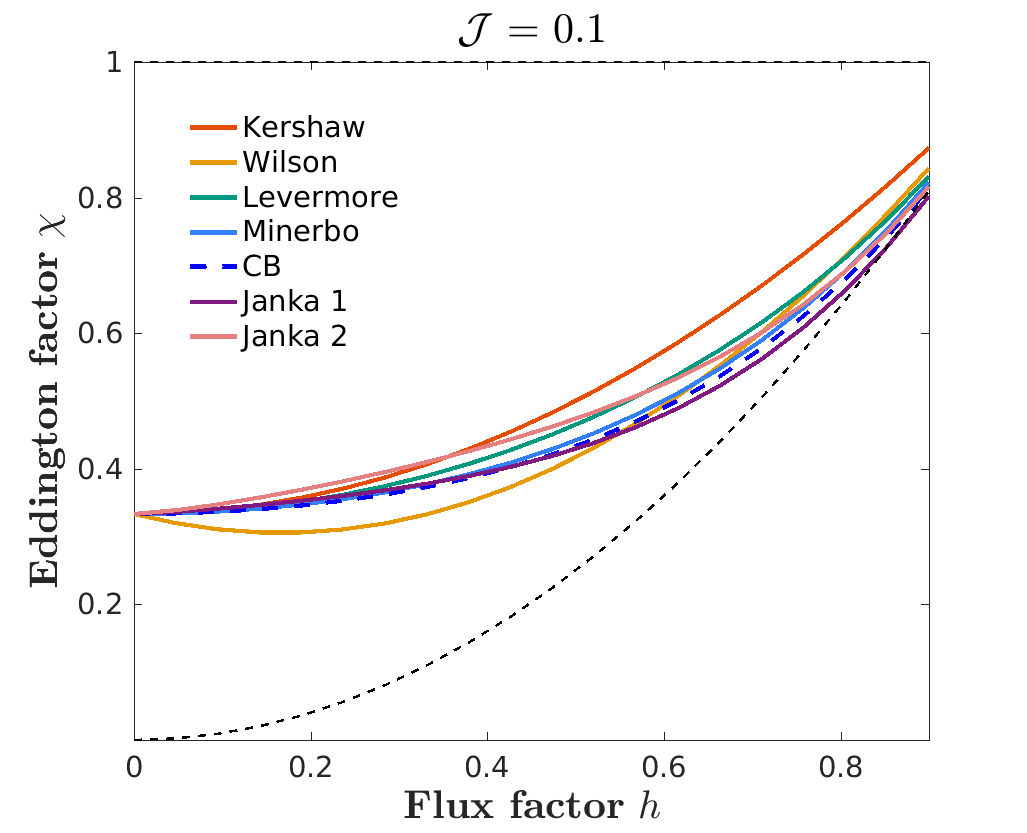
\includegraphics[width=0.5\textwidth]{figures/Closures0_10}
    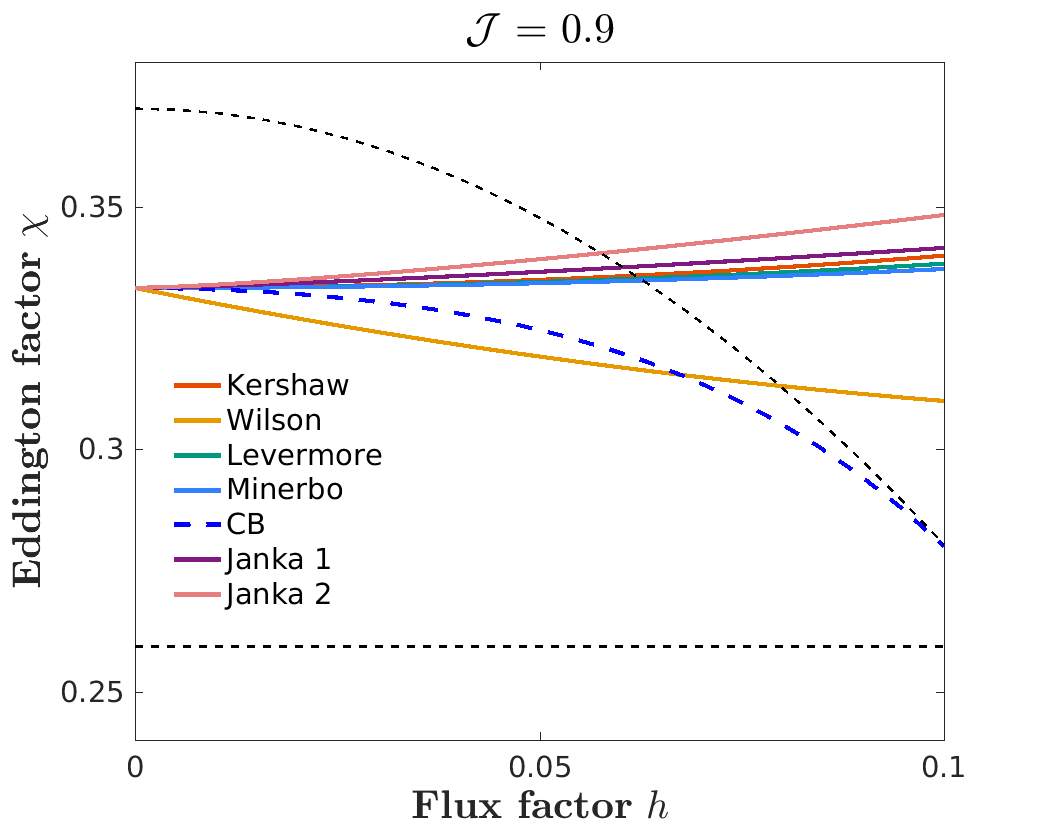
\includegraphics[width=0.5\textwidth]{figures/Closures0_90}
  \end{tabular}
   \caption{Plot of Eddington factors $\chi$ versus flux factor $h$ for different values of $\cJ$ for various algebraic closures: $\cJ=0.1$ (left panel, low occupancy) and $\cJ=0.9$ (right panel, high occupancy).  In each panel we plot the Eddington factors of two-moment closures due to Kershaw (red), Wilson (yellow), Levermore (green), Minerbo (light blue), Cernohorsky \& Bludman (blue), Janka~1 (purple), and Janka~2 (pink) .  We also plot $\chi_{\mbox{\tiny min}}$ and $\chi_{\mbox{\tiny max}}$, defined in Eq.~\eqref{eq:eddingtonFactorBounds} (lower and upper dashed black lines, respectively).}
  \label{fig:EddingtonFactorsWithDifferentClosure}
\end{figure}